\documentclass[12pt]{article}
\setlength{\oddsidemargin}{0in}
\setlength{\evensidemargin}{0in}
\setlength{\textwidth}{6.5in}
\setlength{\parindent}{0in}
\setlength{\parskip}{\baselineskip}
\usepackage{amsmath,amsfonts,amssymb}
\usepackage{graphicx}
\usepackage{enumitem}
\usepackage[]{algorithmicx}
\usepackage{amsthm}
\usepackage{fancyhdr}
\pagestyle{fancy}
\setlength{\headsep}{36pt}
\usepackage{tkz-berge}
\usetikzlibrary{positioning, automata}

\usepackage{hyperref}

\theoremstyle{remark}
\newtheorem*{solution}{Solution}

\newcommand{\makenonemptybox}[2]{%
%\par\nobreak\vspace{\ht\strutbox}\noindent
\item[]
\fbox{% added -2\fboxrule to specified width to avoid overfull hboxes
% and removed the -2\fboxsep from height specification (image not updated)
% because in MWE 2cm is should be height of contents excluding sep and frame
\parbox[c][#1][t]{\dimexpr\linewidth-2\fboxsep-2\fboxrule}{
  \hrule width \hsize height 0pt
  #2
 }%
}%
\par\vspace{\ht\strutbox}
}
\makeatother

\begin{document}
\definecolor {processblue}{cmyk}{0.96,0,0,0}

\lhead{{\bf CSCI 3104, Algorithms \\ Problem Set 3b (50 points)} }
\rhead{Name: Luna McBride \\ ID: 107607144 \\ {\bf Profs.\ Hoenigman \& Agrawal\\ Fall 2019, CU-Boulder}}
\renewcommand{\headrulewidth}{0.5pt}

\phantom{Test}

\begin{small}
\textbf{Instructions for submitting your solution}:
\vspace{-5mm} 

\begin{itemize}
	\item The solutions \textbf{should be typed} and we cannot accept hand-written solutions. \href{http://ece.uprm.edu/~caceros/latex/introduction.pdf}{Here's a short intro to Latex.}
	\item You should submit your work through \href{https://www.gradescope.com/courses/59294}{\textbf{Gradescope}} only.
	\item If you don't have an account on it, sign up for one using your CU email. You should have gotten an email to sign up. If your name based CU email doesn't work, try the identikey@colorado.edu version. 
	\item Gradescope will only accept \textbf{.pdf} files (except for code files that should be submitted separately on Gradescope if a problem set has them) and \textbf{try to fit your work in the box provided}. 
	\item You cannot submit a pdf which has less pages than what we provided you as Gradescope won't allow it. 
	\item Verbal reasoning is typically insufficient for full credit. Instead, write a logical argument, in the style of a mathematical proof.
	\item For every problem in this class, you must justify your answer:\ show how you arrived at it and why it is correct. If there are assumptions you need to make along the way, state those clearly.
	
	\item You may work with other students. However, \textbf{all solutions must be written independently and in your own words.} Referencing solutions of any sort is strictly prohibited. You must explicitly cite any sources, as well as any collaborators. 
\end{itemize}



\vspace{-4mm} 
\end{small}

\hrulefill

\newpage
\begin{enumerate}

\item (23 pts) Imagine an alternate reality where CU has a small robot that travels around the campus delivering food to hungry students. The robot starts at the C4C and goes to whatever dorm or classroom has placed the order. The fully-charged battery of the robot has enough energy to travel $k$ meters. On campus, there are $n$ wireless charging pods where the robot can stop to charge its battery. Denote by $l_1 < l_2 < \cdots < l_n$  the locations of the charging pods along the route with $l_i$ the distance from the C4C to the $i${\em th} charging pod. The distance between neighboring charging pods is assumed to be at most $k$ meters. Your objective is to make as few charging stops as possible along the way. 
\begin{enumerate}
\item (10 pts) Write a python program for an optimal greedy algorithm to determine at which charging pods the robot would stop. Your code should take as input $k$ and a \textit{list} of distances of charging pods (first distance in the list is 0 to represent the start point and the last is the destination and not a pod). Print out the charging pods where the robot stops using your greedy strategy.\\
Example 1 - If \textbf{k = 40} and \textbf{Pods = [0, 20, 37, 54, 70, 90]}. Number of stops required is 2 and the output should be \textbf{[37, 70]}.\\
Example 2 - If \textbf{k = 20} and \textbf{Pods = [0, 18, 21, 24, 37, 56, 66]}. Number of stops required is 3 and the output should be \textbf{[18, 37, 56]}.\\
Example 3 - If \textbf{k = 20} and \textbf{Pods = [0, 10, 15, 18]}. Number of stops required is 0 and the output should be \textbf{[]}.\\



% Give an optimal greedy algorithm to determine at which charging stations you would stop. 
\item (3 pts) Provide the time complexity of your python algorithm, including an explanation.
\begin{solution}
$\newline$ p=k$-->$1, c=len(stations) $-->$1, stops=np.zeros(0,dtype=int)$-->$1 $\newline$ count=0$--> 1 \newline$ for i in range (1,c): $-->$ c (only c because the +1 from rechecking the loop is negated by a -1 of not starting at 0) $\newline$ Statements in loop: 5 (for worst case) $\newline$ return count, stops $-->$1 $\newline \newline$ Constants (non-loop): 5, non-constants (from loop): $5c$ $\newline$ $5c+5$ $\newline \mathcal{O}(c)$
\end{solution}
\pagebreak
\item (10 pts) Prove that your algorithm gives an optimal solution.
\begin{solution}
$\newline$ Let $i_1$...$i_n$ be the list of charge stations in the algorithm, len(A)=n $\newline$ Let $j_1$...$j_m$ be the list of charge stations in the optimal solution, len(O)=m $\newline \newline$ Base case: For s=1, there is one station. $\newline$ ----Case 1: The destination is within battery life, neither optimal nor algorithm needs to stop at a charging station. $\newline$ ----Case 2: The destination is not within battery life, in which both will need to charge at the station to reach the destination. $\newline \newline$ Inductive Hypothesis: Assume $i_s$=$j_s$, where s is the station they both share a recharge point at. $\newline \newline$ Inductive Step: Following how this question was defined, the optimal and algorithm bot both have an endpoint and start point at the same distance. The most optimal way to go about this is to go the furthest possible before recharging again, as to maximize battery life. That is, $j_{s+1}$=$j_s <$ Max(O[rs]) $\leq$ k+$j_s$, where rs is the random station we are checking and Max(O[rs]) is the furthest station less than or equal to k+$j_s$. $\newline$ The algorithm I coded does the same calculation, using a variable p. p=$i_s$+k and is used to search for the highest value that does not fit in the range from the last station. The one before must be the furthest station available in the range of the battery life, as the one after it in the list exceeded the distance. Since the optimal and my algorithm both check and get the absolute furthest value, with the same set of data, the absolute furthests must be the same for the given battery life. That is to say, $j_{s+1}=i_{s+1}$. $\newline \newline$ Therefore, by weak induction, this algorithm is an optimal solution.
\end{solution}
\end{enumerate}
\pagebreak

\item (7 pts) Using Dijkstra's algorithm, determine the length of the shortest path from $v_{0}$ to each of the other vertices in the graph. Clearly specify the distances from $v_{0}$ to each vertex \textbf{after each iteration} of the algorithm.
\begin{center}
	\begin {tikzpicture}[-latex ,auto ,node distance =2 cm and 3cm ,on grid ,
	semithick ,
	state/.style ={ circle ,top color =white , bottom color = processblue!20 ,
	draw,processblue , text=blue , minimum width =1 cm}]

	\node[state] (A) {$v_{0}$};
	\node[state] (B) [above right = of A] {$v_{1}$};
	\node[state] (C) [below right = of A] {$v_{2}$};
	\node[state] (D) [right = of B] {$v_{3}$};
	\node[state] (E) [right = of C] {$v_{4}$};
	\node[state] (F) [below right = of D] {$v_{5}$};
	\path (A) edge node[above] {$2$} (B);
	\path (A) edge node[right] {$7$} (C);
	\path (B) edge node[right] {$4$} (C);
	\path (B) edge node[above] {$3$} (D);
	\path (B) edge node[right] {$1$} (E);
	\path (C) edge node[above] {$6$} (E);
	\path (E) edge node[right] {$1$} (D);
	\path (D) edge node[above] {$13$} (F);
	\path (E) edge node[above] {$19$} (F);

	\path (C) edge [bend right = 50] node[below] {$3$} (F);
	
	\end{tikzpicture}  
\end{center}
\begin{solution}
$ \newline 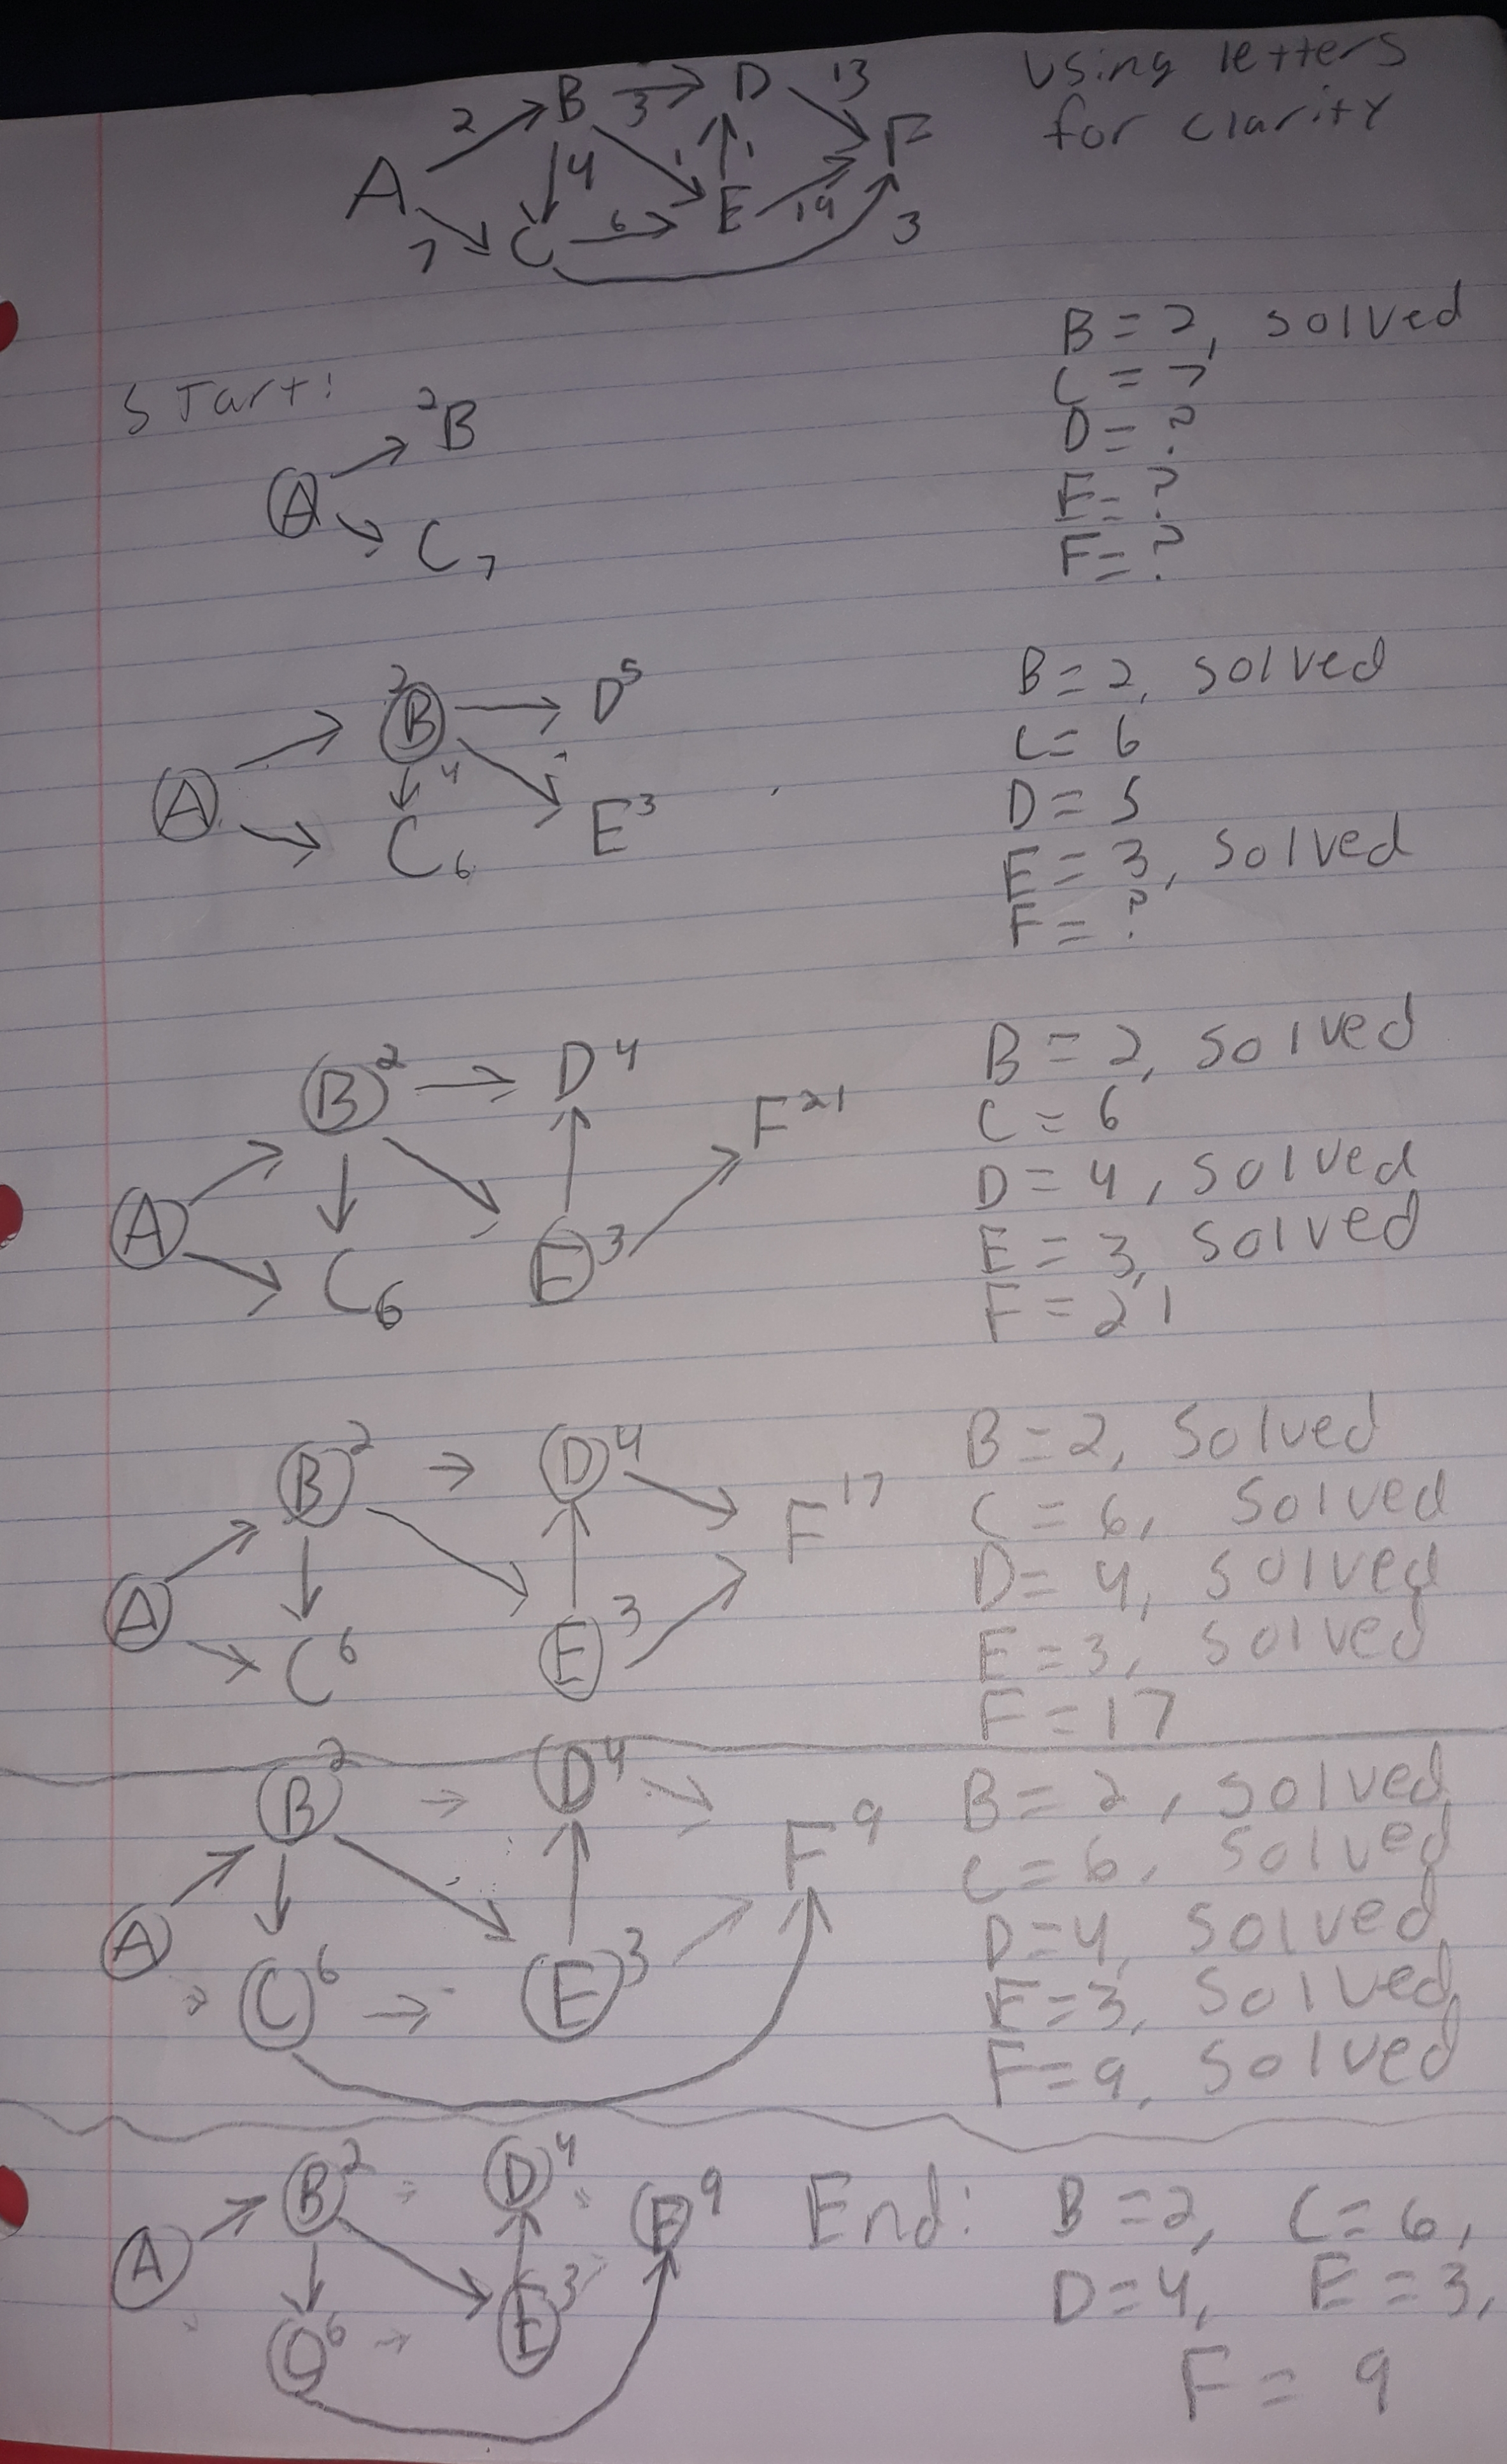
\includegraphics[width=\textwidth, height=7.5in]{Dijkstra}$
\end{solution}
\pagebreak


\item (20 pts) After years of futility, the Colorado Rockies have decided to try a new approach to signing players. Next year, they have a target number of wins, $n$, and they want to sign the fewest number of players who can produce exactly those $n$ wins. In this model, each player has a win value of $v_{1}<v_{2}<\dots<v_{r}$ for $r$ player types, where each player's value $v_{i}$ is a positive integer representing the number of wins he brings to the team. (Note: In a real-world example, All-Star third baseman, Nolan Arenado, contributed 4.5 wins this year beyond what a league-minimum player would have contributed to the team.) 
The team's goal is to obtain a set of counts $\{d_{i}\}$, one for each player type (so $d_{i}$ represents the quantity of players with valuation $v_{i}$ that are recruited), such that $\sum_{i=1}^{r}d_{i}=k$ and where $k$ is the number of players signed, and $k$ is minimized.
	\begin{enumerate}
	\item  (10 pts) Write a greedy algorithm that will produce an optimal solution for a set of player win values of $[1, 2, 4, 8, 16]$ and prove that your algorithm is optimal for those values. Your algorithm need only be optimal for the fixed win values $[1, 2, 4, 8, 16]$. You do \textbf{not} need to consider other configuration of win values.
	\begin{solution}
$\newline$ (Code in python code file) $\newline \newline$ The code has a big O of n, as the loop creates a multiplier of n while all other items remain as constants $\newline$ The optimal searches the list of items for the specific values [1,2,4,8,16] and checks specifically if those are already chosen. The minimized player count will then be the chosen based off only one instance of each, putting just as many players as there are instances of each value.  $\newline$ This is what my code does, as it looks specifically for these values specifically, using numpy to easily check the values in the array and the math log function to get the index of the array for already used values. With the values coming out the same and being specifically taylored to this set of values, there is no doubt that this is an optimal algorithm for this playerbase.
    \end{solution}
    \pagebreak

[Additional space for solving Q3a]
\pagebreak

\item (10 pts) Find a set of win values where your algorithm does not produce the optimal solution and show where your algorithm fails for those values. 
\begin{solution}
$\newline$ As this algorithm is heavily tuned to the values [1,2,4,8,16], there is a lot to be desired for other values. Of course, there is the basic things (array counting already used values only going up to 5, for example), but that is to be expected from code like this in general. However, there are more parts that could break under any other value. $\newline$ if l in values: --$>$ This if checks if the value given is in the list of given values. This will trip up for any value not provided specifically in the list, such as 3 and 5. $\newline$ p=int(math.log(l,2)), and subsequently if used[p]==1: --$>$ The value p is set up to be specifically used as to not have to index through the array of listed values for keeping track of used values. Since the values [1,2,4,8,16] are all $2^n$, it was easier to just log the 2 out to get the indecies than to loop through the set of necessary values. Of course, this could work out for anything else that follows the $2^n$ structure, however, this vastly neglects values like 3, 5, or any other value that is not of that form. I would have to restructure everything and maybe add another loop to make up for that issue. $\newline$ Not to add more to the pile, but if we added decimal values in there in addition, it would turn into a nightmare. Perhaps a floor/ceiling function could be used to put those into regular numbers, but that would be disingenuous for us to do given the nature of these averaged wins. $\newline \newline$ Of course, a lot more could be done to make this optimal for all values, however, in its current state, this algorithm would not only be unoptimal for values outside our list, it would just flat out not work for anything outside the [1,2,4,8,16] range. It is easy to make something super optimal for just one thing like we have done here, but giving it new tricks will completely destroy the whole function if made too crazy optimal.
\end{solution}

    \end{enumerate}

\end{enumerate}

\pagebreak
\textbf{Ungraded questions} - These questions are for your practice. We won't grade them or provide a typed solution but we are open to discuss these in our OHs and you should take feed backs on your approach during the OHs. These questions are part of the syllabus. 

\begin{enumerate}

\item Suppose we have a directed graph $G$, where each edge $e_{i}$ has a weight $w_{i} \in (0, 1).$  The weight of a path is the product of the weights of each edge. 
\begin{enumerate}[label=(\alph*)]
\item Explain why a version of Dijkstra's algorithm cannot be used here. [\textbf{Hint:} We may think about transforming $G$ into a graph $H$, where the weight of edge $i$ in $H$ is $\ln(w_{i})$. It is equivalent to apply Dijkstra's algorithm to $H$.]
\begin{solution}

\end{solution}

\item What conditions does each edge weight $w_{i}$ need to satisfy, in order to use Dijkstra's algorithm?
\begin{solution}

\end{solution}


\end{enumerate}



\end{enumerate}

\end{document}
